\documentclass[twocolumn]{article}
\usepackage{graphicx}
\usepackage{url}
\usepackage[spanish]{babel}
\selectlanguage{spanish}
\usepackage[utf8]{inputenc}
\usepackage{amsmath}

\title{Tarea 2}
\author{Miguel~Angel~Asencio~Hurtado, Ana~María~Rodríguez~Reyes}

\begin{document}
\maketitle
\textbf{1. Desarrollar en series de Fourier}

$$f(t) = t^2,\; -\pi \leq t \leq \pi$$

\textbf{R/} Se plantea la serie de fourier de la siguiente manera:

$$f(t) = \frac{a_0}{2} + \sum_{n=1}^\infty\left(a_n\,cos(n\omega_0t) + b_n\,sin(n\omega_0t)\right)$$

Por lo que los coeficientes $a_x$ se pueden definir de la siguiente forma:
\begin{eqnarray*}
a_0 &=& \frac{2}{T}\int_{-T/2}^{T/2}f(t)dt\\
a_n &=& \frac{2}{T}\int_{-T/2}^{T/2}f(t)cos(n\omega_0t)dt\\
b_n &=& \frac{2}{T}\int_{-T/2}^{T/2}f(t)sin(n\omega_0t)dt
\end{eqnarray*}

Reemplazando por las variables del enunciado se llega a:
\begin{eqnarray*}
a_0 &=& \frac{1}{\pi}\int_{-\pi}^{\pi}t^2dt\\
a_n &=& \frac{1}{\pi}\int_{-\pi}^{\pi}t^2cos(n\,t)dt\\
b_n &=& \frac{1}{\pi}\int_{-\pi}^{\pi}t^2sin(n\,t)dt
\end{eqnarray*}

Resolviendo para $a_0$:
\begin{eqnarray*}
a_0 &=& \frac{1}{\pi}\int_{-\pi}^{\pi}t^2dt\\
&=& \frac{1}{\pi} \frac{t^3}{3}\bigg|_{t=-\pi}^{\pi}\\
&=& \frac{1}{3\pi} (\pi^3 - (-\pi)^3)\\
&=& \frac{2}{3}\pi^2
\end{eqnarray*}

Resolviendo para $a_n$:
\begin{eqnarray*}
a_n &=& \frac{1}{\pi}\int_{-\pi}^{\pi}t^2cos(n\,t)dt\\
&=& \frac{1}{\pi} \left(\frac{t^2sin(n\,t)}{n} + \frac{2t\,cos(n\,t)}{n^2} - \frac{2\,sin(n\,t)}{n^3}\right)\bigg|_{t=-\pi}^{\pi}\\
&=& \frac{\pi^2sin(n\,\pi)}{n\pi} + \frac{2\pi\,cos(n\,\pi)}{n^2\pi} - \frac{2\,sin(n\,\pi)}{n^3\pi}\\
& &- \frac{\pi^2sin(n(-\pi))}{n\pi} + \frac{2\pi\,cos(n(-\pi))}{n^2\pi} + \frac{2\,sin(n(-\pi))}{n^3\pi}\\
&=& 2\pi^2 sinc(n\,\pi) + \frac{4\pi}{n}cosc(n\,\pi) - \frac{4}{n^2}sinc(n\,\pi)
\end{eqnarray*}

Resolviendo para $b_n$:
\begin{eqnarray*}
b_n &=& \frac{1}{\pi}\int_{-\pi}^{\pi}t^2sin(n\,t)dt\\
&=& \frac{1}{\pi} \left(-\frac{t^2cos(n\,t)}{n} - \frac{2t\,sin(n\,t)}{n^2} + \frac{2\,cos(n\,t)}{n^3}\right)\bigg|_{t=-\pi}^{\pi}\\
&=& -\frac{\pi^2cos(n\,\pi)}{n\pi} - \frac{2\pi\,sin(n\,\pi)}{n^2\pi} + \frac{2\,cos(n\,\pi)}{n^3\pi}\\
& &+ \frac{\pi^2cos(n(-\pi))}{n\pi} - \frac{2\pi\,sin(n(-\pi))}{n^2\pi} - \frac{2\,cos(n(-\pi))}{n^3\pi}\\
&=& 0
\end{eqnarray*}

De manera que la serie de Fourier de $f(t)$ queda de la siguiente forma:
\begin{eqnarray*}
f(t) &=& \frac{\pi^2}{3} + \sum_{n=1}^\infty\left(a_n\,cos(n\,t)\right)\\
a_n &=& \left(2\pi^2  - \frac{4}{n^2} \right) sinc(n\,\pi) + \frac{4\pi}{n}cosc(n\,\pi)
\end{eqnarray*}

Esta progresión puede verse en la Figura~\ref{fig_1}, en donde a medida que se agrega un término esta sumatoria se aproxima a la señal original (mostrada en azul).

\begin{figure}[!t]
\centering
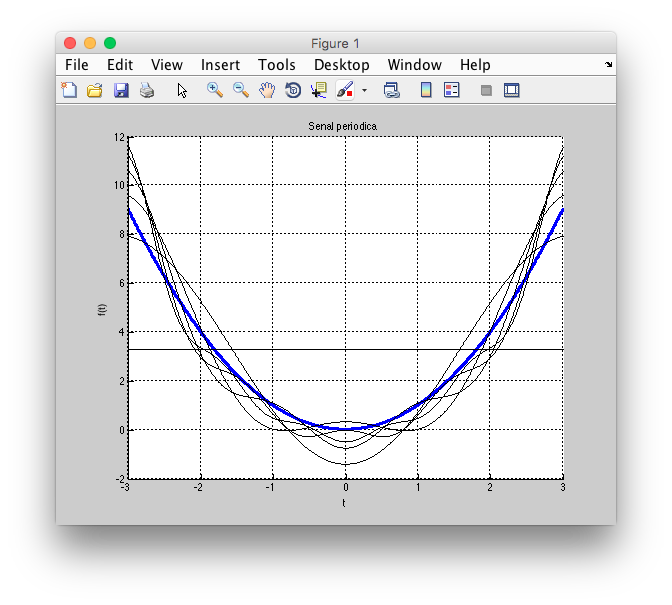
\includegraphics[width=3.5in]{imgs/sqrt.png}
\caption{Señal $f(t) = t^2$}
\label{fig_1}
\end{figure}

Los primeros cinco armónicos de esta serie son:

\begin{eqnarray*}
A_1 &=& \frac{\pi^2}{3} - 4\cos{(t)} \\
A_2 &=& \frac{\pi^2}{3} + \cos{(2t)} \\
A_3 &=& \frac{\pi^2}{3} - \frac{4}{9}\cos{(3t)} \\
A_4 &=& \frac{\pi^2}{3} + \frac{1}{4}\cos{(4t)} \\
A_5 &=& \frac{\pi^2}{3} - \frac{4}{25}\cos{(5t)}
\end{eqnarray*}

La serie se puede expresar como:

$$f(t) = \frac{\pi^2}{3} + 4 \sum_{n=1}^\infty\left(\frac{(-1)^n}{n^2}\cos{(n\,t)}\right)$$

\textbf{2. Desarrollar en series de Fourier}

$$f(t) = t \, sin(t),\; -\pi \leq t \leq \pi$$


\textbf{R/} Se plantea la serie de Fourier de la siguiente manera:

$$f(t) = \frac{a_0}{2} + \sum_{n=1}^\infty\left(a_n\,cos(n\omega_0t) + b_n\,sin(n\omega_0t)\right)$$

Por lo que los coeficientes $a_x$ se pueden definir de la siguiente forma:
\begin{eqnarray*}
a_0 &=& \frac{2}{T}\int_{-T/2}^{T/2}f(t)dt\\
a_n &=& \frac{2}{T}\int_{-T/2}^{T/2}f(t)cos(n\omega_0t)dt\\
b_n &=& \frac{2}{T}\int_{-T/2}^{T/2}f(t)sin(n\omega_0t)dt
\end{eqnarray*}

Reemplazando por las variables del enunciado se llega a:
\begin{eqnarray*}
a_0 &=& \frac{1}{\pi}\int_{-\pi}^{\pi}tsin(t)dt\\
a_n &=& \frac{1}{\pi}\int_{-\pi}^{\pi}tsin(t)cos(n\,t)dt\\
b_n &=& \frac{1}{\pi}\int_{-\pi}^{\pi}tsin(t)sin(n\,t)dt
\end{eqnarray*}

Resolviendo para $a_0$:
\begin{eqnarray*}
a_0 &=& \frac{1}{\pi}\int_{-\pi}^{\pi}tsin(t)dt\\
&=& \frac{1}{\pi} \bigg[ sin(t) -tcos(t)\bigg|_{t=-\pi}^{0} + sin(t) -tcos(t)\bigg|_{t=0}^{\pi} \bigg] \\
&=& \frac{1}{\pi} [2\pi]\\
&=& 2
\end{eqnarray*}

Resolviendo para $a_n$:
\begin{eqnarray*}
a_n &=& \frac{1}{\pi}\int_{-\pi}^{\pi}tsin(t)cos(n\,t)dt\\
&=& \frac{1}{\pi} \bigg(\frac{1}{2}\bigg(-\frac{sin((n-1)t)}{(n-1)^{2}} + \frac{sin((n+1)t)}{(n+1)^{2}}+ \\
& & \frac{tcos((n-1)t)}{n-1} - \frac{tcos((n+1)t)}{n+1})\bigg)\bigg)\bigg|_{t=-\pi}^{\pi}\\
&=& \frac{4nsin(\pi n)-2\pi(n^{2}-1)cos(\pi n))}{\pi(n^{2}- 1)^{2}}\\
\end{eqnarray*}

Resolviendo para $b_n$:
\begin{eqnarray*}
b_n &=& \frac{1}{\pi}\int_{-\pi}^{\pi}tsin(t)sin(n\,t)dt\\
&=& \frac{1}{\pi} \bigg[\frac{1}{(n^{2}-1)^{2}}(sin(t)((n^{2}+1)sin(nt) \\
& & -n(n^{2}-1)xcos(nx))+ \\
& & cos(t)((n^{2}-1)xsin(nx) + \\
& &2ncos(nx)))\bigg]\bigg|_{t=-\pi}^{\pi}\\
&=& 0
\end{eqnarray*}

De manera que la serie de Fourier de $f(t)$ queda de la siguiente forma:
\begin{eqnarray*}
f(t) &=& 1 + \sum_{n=1}^\infty\left(a_n\,cos(n\,t)\right)\\
a_n &=& \frac{4nsin(\pi n)-2\pi(n^{2}-1)cos(\pi n)}{\pi(n^{2}- 1)^{2}}
\end{eqnarray*}

Esta progresión puede verse en la Figura~\ref{fig_1b}, en donde a medida que se agrega un término esta sumatoria se aproxima a la señal original (mostrada en azul).

\begin{figure}[!t]
\centering
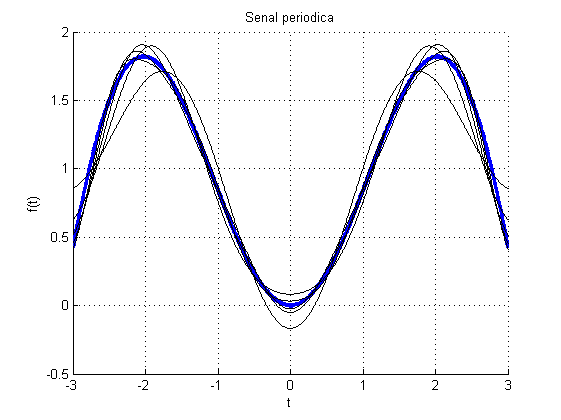
\includegraphics[width=3.5in]{imgs/tsint.png}
\caption{Señal $f(t) = tsin(t)$}
\label{fig_1b}
\end{figure}

Los primeros cinco armónicos de esta serie son:

\begin{eqnarray*}
A_1 &=& \frac{-cos(t)}{2} \\
A_2 &=& \frac{-2}{3} cos(2t) \\
A_3 &=& \frac{1}{4} cos(3t) \\
A_4 &=& \frac{-2}{15} cos(4t) \\
A_5 &=& \frac{1}{12} cos(5t)
\end{eqnarray*}

La serie se puede expresar como:

$$f(t) = 1 - \frac{cos(t)}{2} + \sum_{n=2}^\infty\left( \frac{2(-1)^{n+1}}{n^2 - 1} \,cos(n t) \right)$$

Utilizando la forma compleja de la serie de Fourier:


$$f(t) =  \sum_{n=-\infty}^\infty c_n e^{jn\omega_0t} $$


Por lo que el coeficiente $c_n$ se puede definir de la siguiente forma:
\begin{eqnarray*}
c_n &=& \frac{1}{T}\int_{-T/2}^{T/2}f(t)e^{-jn\omega_0t}dt
\end{eqnarray*}

Reemplazando por las variables del enunciado se llega a:

\begin{eqnarray*}
c_n &=& \frac{1}{2\pi}\int_{-\pi}^{\pi}tsin(t)e^{-jn\omega_0t}dt
\end{eqnarray*}

Resolviendo para $c_n$:
\begin{eqnarray*}
c
_n &=& \frac{1}{2\pi}\int_{-\pi}^{\pi}tsin(t)e^{-jn\omega_0t}dt\\
&=& \frac{1}{2\pi}\int_{-\pi}^{\pi}t \frac{e^{jt} -e^{-jt}}{2j} e^{-jn\omega_0t}dt\\
& & \frac{tcos((n-1)t)}{n-1} - \frac{tcos((n+1)t)}{n+1})\bigg)\bigg)\bigg|_{t=-\pi}^{\pi}\\
&=& \frac{4nsin(\pi n)-2\pi(n^{2}-1)cos(\pi n)}{\pi(n^{2}- 1)^{2}}\\
\end{eqnarray*}

Cinco armónicos de la serie compleja son:

\begin{eqnarray*}
A_{-2} &=& \frac{-1}{3} e^{-2 j t} \\
A_{-1} &=& \frac{-1}{4} e^{-1 j t} \\
A_0 &=& 1 \\
A_1 &=& \frac{-1}{4} e^{1 j t}\\
A_2 &=& \frac{-1}{3} e^{2 j t} 
\end{eqnarray*}


\textbf{3. Desarrollar en series de Fourier}

$$f(t) = t,\; -\pi \leq t \leq \pi$$

\textbf{R/} Se plantea la serie de fourier de la siguiente manera:

$$f(t) = \frac{a_0}{2} + \sum_{n=1}^\infty\left(a_n\,cos(n\omega_0t) + b_n\,sin(n\omega_0t)\right)$$

Por lo que los coeficientes $a_x$ se pueden definir de la siguiente forma:
\begin{eqnarray*}
a_0 &=& \frac{2}{T}\int_{-T/2}^{T/2}f(t)dt\\
a_n &=& \frac{2}{T}\int_{-T/2}^{T/2}f(t)cos(n\omega_0t)dt\\
b_n &=& \frac{2}{T}\int_{-T/2}^{T/2}f(t)sin(n\omega_0t)dt
\end{eqnarray*}

Reemplazando por las variables del enunciado se llega a:
\begin{eqnarray*}
a_0 &=& \frac{1}{\pi}\int_{-\pi}^{\pi}t\,dt\\
a_n &=& \frac{1}{\pi}\int_{-\pi}^{\pi}t\,cos(n\,t)dt\\
b_n &=& \frac{1}{\pi}\int_{-\pi}^{\pi}t\,sin(n\,t)dt
\end{eqnarray*}

Resolviendo para $a_0$:
\begin{eqnarray*}
a_0 &=& \frac{1}{\pi}\int_{-\pi}^{\pi}t\,dt\\
&=& \frac{1}{\pi} \frac{t^2}{2}\bigg|_{t=-\pi}^{\pi}\\
&=& \frac{1}{2\pi} (\pi^2 - (-\pi)^2)\\
&=& 0
\end{eqnarray*}

Resolviendo para $a_n$:
\begin{eqnarray*}
a_n &=& \frac{1}{\pi}\int_{-\pi}^{\pi}t\,cos(n\,t)dt\\
&=& \frac{1}{\pi} \left(\frac{t\,sin(n\,t)}{n} + \frac{cos(n\,t)}{n^2}\right)\bigg|_{t=-\pi}^{\pi}\\
&=& \frac{\pi\,sin(n\,\pi)}{n\pi} + \frac{cos(n\,\pi)}{n^2\pi}\\
& &- \frac{(-\pi)sin(n(-\pi))}{n\pi} - \frac{cos(n(-\pi))}{n^2\pi}\\
&=& 0
\end{eqnarray*}

Resolviendo para $b_n$:
\begin{eqnarray*}
b_n &=& \frac{1}{\pi}\int_{-\pi}^{\pi}t\,sin(n\,t)dt\\
&=& \frac{1}{\pi} \left(-\frac{t\,cos(n\,t)}{n} + \frac{sin(n\,t)}{n^2}\right)\bigg|_{t=-\pi}^{\pi}\\
&=& -\frac{\pi\,cos(n\,\pi)}{n\pi} + \frac{sin(n\,\pi)}{n^2\pi}\\
& & + \frac{(-\pi)cos(n(-\pi))}{n\pi} - \frac{sin(n(-\pi))}{n^2\pi}\\
&=& \frac{2}{n}sinc(n\,\pi) -2\pi\,cosc(n\,\pi)
\end{eqnarray*}

De manera que la serie de Fourier de $f(t)$ queda de la siguiente forma:
$$f(t) = \sum_{n=1}^\infty\left(\left(\frac{2}{n}sinc(n\,\pi) -2\pi\,cosc(n\,\pi)\right)sin(n\,t)\right)$$

Esta progresión puede verse en la Figura~\ref{fig_3}, en donde a medida que se agrega un término esta sumatoria se aproxima a la señal original (mostrada en azul).

\begin{figure}[!t]
\centering
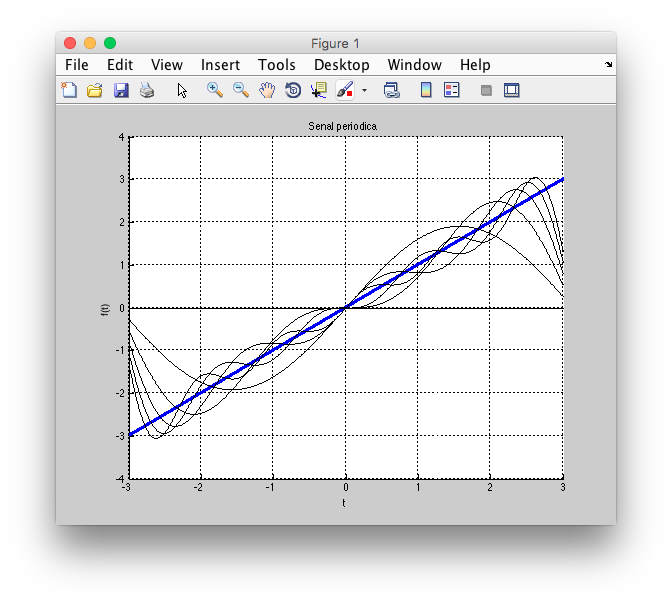
\includegraphics[width=3.5in]{imgs/lin.png}
\caption{Señal $f(t) = t$}
\label{fig_3}
\end{figure}

Los primeros cinco armónicos de esta serie son:

\begin{eqnarray*}
A_1 &=& - 2\sin{(t)} \\
A_2 &=& \sin{(2t)} \\
A_3 &=& - \frac{2}{3}\sin{(3t)} \\
A_4 &=& \frac{1}{2}\sin{(4t)} \\
A_5 &=& - \frac{2}{5}\sin{(5t)}
\end{eqnarray*}

La serie se puede expresar como:

$$f(t) = 2 \sum_{n=1}^\infty\left(\frac{(-1)^n}{n}\sin{(n\,t)}\right)$$

\textbf{4. Desarrollar en series de Fourier}

$$f(t) = \begin{cases}
\pi +t, &-\pi \leq t \leq 0\\
t, &0 < t \leq \pi
\end{cases}$$

\textbf{R/} Se plantea la serie de fourier de la siguiente manera:

$$f(t) = \frac{a_0}{2} + \sum_{n=1}^\infty\left(a_n\,cos(n\omega_0t) + b_n\,sin(n\omega_0t)\right)$$

Por lo que los coeficientes $a_x$ se pueden definir de la siguiente forma:
\begin{eqnarray*}
a_0 &=& \frac{2}{T}\int_{-T/2}^{T/2}f(t)dt\\
a_n &=& \frac{2}{T}\int_{-T/2}^{T/2}f(t)cos(n\omega_0t)dt\\
b_n &=& \frac{2}{T}\int_{-T/2}^{T/2}f(t)sin(n\omega_0t)dt
\end{eqnarray*}

Reemplazando por las variables del enunciado se llega a:
\begin{eqnarray*}
a_0 &=& \frac{1}{\pi} \bigg[ \int_{-\pi}^{0}(\pi + t) dt + \int_{0}^{\pi}t dt \bigg] \\
a_n &=&\frac{1}{\pi} \bigg[ \int_{-\pi}^{0}(\pi + t)cos(n\,t) dt + \int_{0}^{\pi}tcos(n\,t) dt \bigg] \\
b_n &=& \frac{1}{\pi} \bigg[ \int_{-\pi}^{0}(\pi + t)sin(n\,t) dt + \int_{0}^{\pi}tsin(n\,t) dt \bigg]
\end{eqnarray*}

Resolviendo para $a_0$:
\begin{eqnarray*}
a_0 &=& \frac{1}{\pi} \bigg[ \int_{-\pi}^{0}(\pi + t) dt + \int_{0}^{\pi}t dt \bigg]\\
&=& \frac{1}{\pi} \bigg[ \frac{t^{2}}{2} + \pi t\bigg|_{t=-\pi}^{0} + \frac{t^{2}}{2}\bigg|_{t=0}^{\pi} \bigg] \\
&=& \frac{1}{\pi} [\frac{\pi^{2}}{2} + \frac{\pi^{2}}{2}]\\
&=& \pi
\end{eqnarray*}

Resolviendo para $a_n$:
\begin{eqnarray*}
a_n &=& \frac{1}{\pi} \bigg[ \int_{-\pi}^{0}(\pi + t)cos(n\,t) dt + \int_{0}^{\pi}tcos(n\,t) dt \bigg] \\
&=& \frac{1}{\pi} \bigg[ \bigg(\frac{cos(n t)}{n^{2}} + \frac{t sin(n t)}{n} + \frac{\pi sin(n t)}{n}\bigg)\bigg|_{t=-\pi}^{0}\\
& & + \bigg(\frac{cos(nt)}{n^{2}} + \frac{tsin(n t)}{n}\bigg)\bigg|_{t=0}^{\pi} \bigg] \\
&=& \frac{1}{\pi} \bigg[ \frac{1 - cos(\pi n)}{n^{2}}+ \frac{\pi n sin(\pi n)+ cos(\pi n) -1}{n^{2}} \bigg]\\
&=& \frac{sin(\pi n)}{n}
\end{eqnarray*}

Resolviendo para $b_n$:
\begin{eqnarray*}
b_n &=&  \frac{1}{\pi} \bigg[ \int_{-\pi}^{0}(\pi + t)sin(n\,t) dt + \int_{0}^{\pi}tsin(n\,t) dt \bigg] \\
&=&  \frac{1}{\pi} \bigg[ \bigg(\frac{sin(n t)}{n^{2}} - \frac{tcos(n t)}{n} - \frac{\pi cos(n t)}{n}\bigg)\bigg|_{t=-\pi}^{0}\\
& & \bigg(\frac{sin(n t)}{n^{2}} - \frac{tcos(n t)}{n}\bigg)\bigg|_{t=0}^{\pi} \bigg] \\
&=& \frac{1}{\pi} \bigg[ \frac{sin(\pi n)-\pi n}{n^{2}} + \frac{sin(\pi n)-\pi n cos(\pi n)}{n^{2}} \bigg]\\
&=& \frac{2sin(\pi n)-\pi n cos(\pi n) - \pi n}{\pi n^{2}}
\end{eqnarray*}

De manera que la serie de Fourier de $f(t)$ queda de la siguiente forma:
\begin{eqnarray*}
f(t) &=& \frac{\pi}{2} + \sum_{n=1}^\infty\left(a_n\,cos(n\,t)+ b_n\,sin(n\,t)\right)\\
a_n &=&  \frac{sin(\pi n)}{n} \\
b_n &=&   \frac{2sin(\pi n)-\pi n cos(\pi n) - \pi n}{\pi n^{2}}
\end{eqnarray*}

Esta progresión puede verse en la Figura~\ref{fig_1d}, en donde a medida que se agrega un término esta sumatoria se aproxima a la señal original (mostrada en azul).

\begin{figure}[!t]
\centering
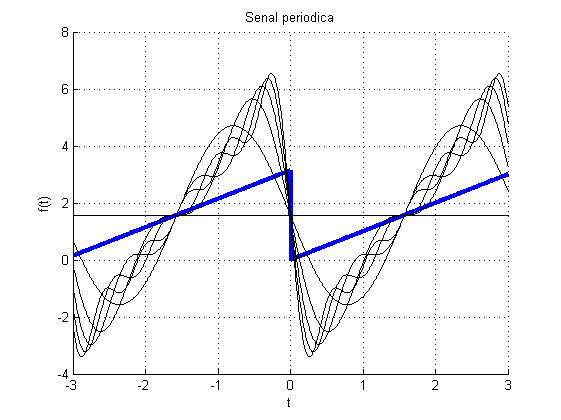
\includegraphics[width=3.5in]{imgs/piece.png}
\caption{Señal $f(t) = \{ \pi +t, t \}$}
\label{fig_1d}
\end{figure}

Los primeros cinco armónicos de esta serie son:

\begin{eqnarray*}
A_1 &=& 0 \\
A_2 &=& - sin(2t) \\
A_3 &=& 0 \\
A_4 &=& \frac{-1}{2} sin(4t) \\
A_5 &=& 0 \\
A_6 &=& \frac{-1}{3} sin(6t) \\
\end{eqnarray*}

Teniendo en cuenta que los armónicos nulos como los impares( $A_1 , A_3,..., A_{2n+1}$) no se tienen en cuenta, la serie se puede representar como:

$$f(t) = \frac{\pi}{2} + \sum_{n=1}^\infty\left( \frac{ -1 \,}{n} \,sin(2 n t) \right)$$


Utilizando la forma compleja de la serie de Fourier:


$$f(t) =  \sum_{n=-\infty}^\infty c_n e^{jn\omega_0t} $$


Por lo que el coeficiente $c_n$ se puede definir de la siguiente forma:
\begin{eqnarray*}
c_n &=& \frac{1}{T}\int_{-T/2}^{T/2}f(t)e^{-jn\omega_0t}dt
\end{eqnarray*}

Reemplazando por las variables del enunciado se llega a:

\begin{eqnarray*}
c_n &=& \frac{1}{2\pi} \left [ \int_{-\pi}^{0}(\pi+t) e^{-jnt}dt + \int_{0}^{\pi}t e^{-jnt}dt \right]
\end{eqnarray*}

Resolviendo para $c_n$:
\begin{eqnarray*}
c_n &=& \frac{1}{2\pi} \left [ \int_{-\pi}^{0}(\pi+t) e^{-jnt}dt + \int_{0}^{\pi}t e^{-jnt}dt \right]\\
&=& \frac{1}{2\pi} \bigg [ \int_{-\pi}^{0}\pi e^{-jnt}dt + \int_{-\pi}^{0}t e^{-jnt}dt + \\
& &  \int_{0}^{\pi}t e^{-jnt}dt \bigg] \\
&=& \frac{1}{2\pi} \bigg [ -\frac{j \pi (-1 + e^{j \pi n})}{n} + \frac{1+e^{j \pi n}(-1 + j \pi n)}{n^2} + \\
& &  \frac{-1+e^{j \pi n}(1 + j \pi n)}{n^2} \bigg] \\
&=& \bigg [ -\frac{j (-1 + e^{j \pi n})}{2n} + \frac{e^{j \pi n}(j)}{ n} \bigg]\\
\end{eqnarray*}

Cinco armónicos para la serie compleja son:

\begin{eqnarray*}
A_{-2} &=& \frac{-j e^{-2 j t}}{2} \\
A_{-1} &=& 0 \\
A_0 &=& \frac{pi}{2} \\
A_1 &=& 0 \\
A_2 &=& \frac{j e^{2 j t}}{2} \\
\end{eqnarray*}

$\,$

\textbf{5. Hallar el periodo}

\textbf{a)} $f(t) = sin(\frac{2\pi}{b-a}t)$

\textbf{R/} El periodo $T$ de una señal senoidal se puede definir como:

$$f(t) = sin\left(\frac{2\pi}{T}t\right)$$

Por lo que para resolver la igualdad:

$$T = (b - a)$$

Es evidente en las Figuras \ref{fig_ba4_2} y \ref{fig_ba5_2} que los periodos coinciden con los calculados.

\begin{figure}[!t]
\centering
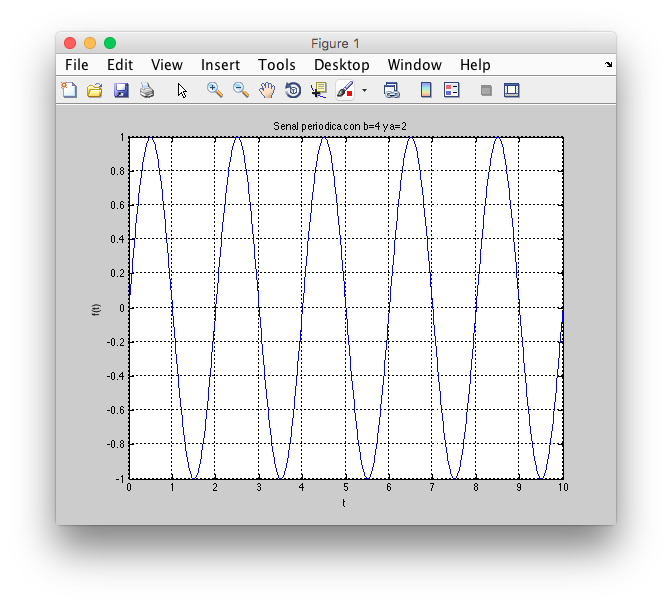
\includegraphics[width=3.5in]{imgs/ba4_2.png}
\caption{Señal $f(t) = sin(\frac{2\pi}{b-a}t)$ con $b=4$ y $a=2$}
\label{fig_ba4_2}
\end{figure}

\begin{figure}[!t]
\centering
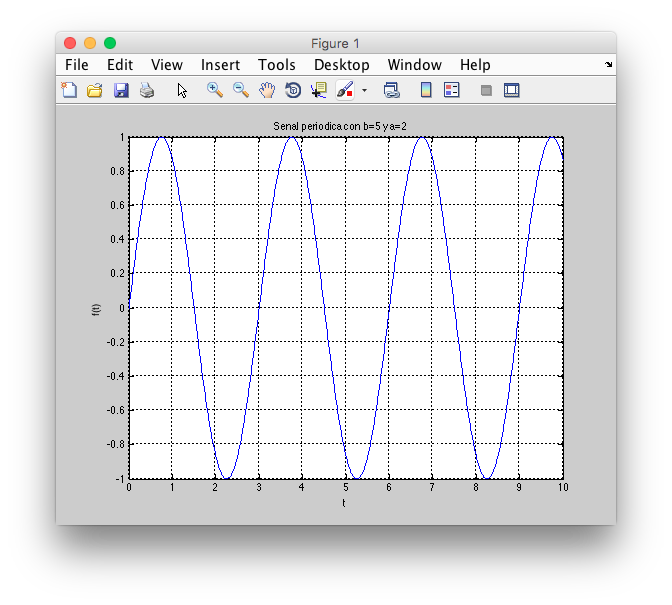
\includegraphics[width=3.5in]{imgs/ba5_2.png}
\caption{Señal $f(t) = sin(\frac{2\pi}{b-a}t)$ con $b=5$ y $a=2$}
\label{fig_ba5_2}
\end{figure}

$\,$

\textbf{b)} $f(t) = sin(t) + \frac{1}{3}sin(3t) + \frac{1}{5}sin(5t)$

\textbf{R/} El periodo $T$ de una señal senoidal se puede definir como:

$$f(t) = sin\left(\frac{2\pi}{T}t\right)$$

Por lo que para cada senoidal su periodo sería:

\begin{eqnarray*}
T_1 &=& 2\pi\\
T_2 &=& \frac{2\pi}{3}\\
T_3 &=& \frac{2\pi}{5}
\end{eqnarray*}

Dado el hecho de que la señal es una señal compuesta, será periódica si el cociente entre sus periodos es un número racional:

\begin{eqnarray*}
\frac{T_1}{T_2} &=& 3\\
\frac{T_1}{T_2} &=& 5\\
\frac{T_2}{T_3} &=& \frac{5}{3}
\end{eqnarray*}

Dado el hecho de que se cumple la condición, la señal es periódica y su periodo será el mínimo común múltiplo de estos periodos:

\begin{eqnarray*}
T &=& m.c.m(T_1,T_2,T_3)\\
&=& m.c.m(2 \pi,2\pi3^{-1},2\pi5^{-1})\\
T &=& 2\pi
\end{eqnarray*}

Es evidente en la Figura \ref{fig_5b} que el periodo coincide con el calculado.

\begin{figure}[!t]
\centering
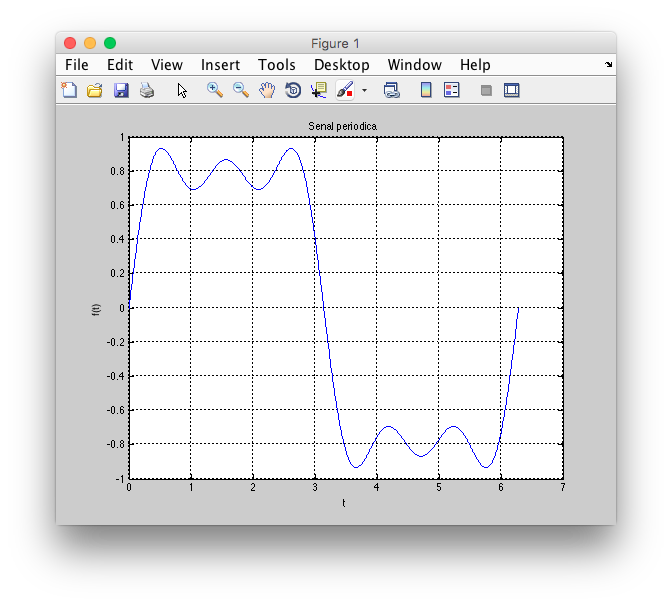
\includegraphics[width=3.5in]{imgs/5b.png}
\caption{Señal $f(t) = sin(t) + \frac{1}{3}sin(3t) + \frac{1}{5}sin(5t)$}
\label{fig_5b}
\end{figure}

$\,$

\textbf{c)} $f(t) = cos(10t) + cos((10+\pi)t)$

\textbf{R/} El periodo $T$ de la función coseno se puede definir como:

$$f(t) = cos\left(\frac{2\pi}{T}t\right)$$

Por lo que para cada coseno su periodo sería:

\begin{eqnarray*}
T_1 &=& \frac{\pi}{5}\\
T_2 &=& \frac{2\pi}{10 + \pi}
\end{eqnarray*}

Dado el hecho de que la señal es una señal compuesta, será periódica si el cociente entre sus periodos es un número racional:

\begin{eqnarray*}
\frac{T_1}{T_2} &=& 1 + \frac{\pi}{10}
\end{eqnarray*}

Dado el hecho de que no se cumple la condición, la señal no es periódica, como se puede observar en la Figura \ref{fig_5c}

\begin{figure}[!t]
\centering
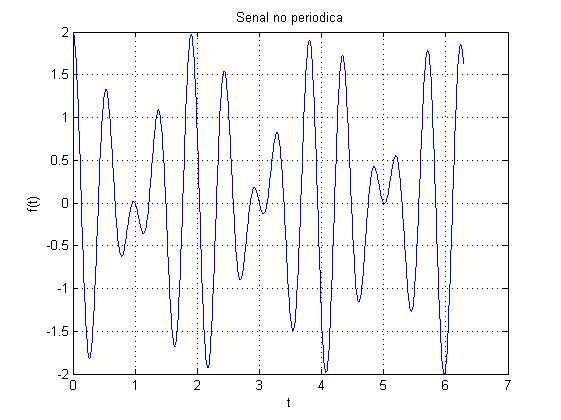
\includegraphics[width=3.5in]{imgs/5c.png}
\caption{Señal $f(t) = cos(10t) + cos((10+\pi)t)$}
\label{fig_5c}
\end{figure}


\end{document}
